
\begin{exercise}

% !TEX root = ../main.tex



\pt{3}\begin{minipage}[t]{.74\linewidth}
	Een massa van \SI{2,0}{kg} bevindt zich in een lift aan een dynamometer. Die laatste duidt een kracht van \SI{10}{N} aan.
\newline
%\newline	
	
	Welke beweging voert de lift uit? Licht toe.
\begin{enumerate}

	\item De lift beweegt naar omlaag met een versnelling van \SI{5,0}{m/s^2}.
	\item De lift beweegt naar omhoog met een versnelling van \SI{5,0}{m/s^2}.
	\item De lift beweegt naar omlaag met een constante snelheid.
	\item De lift beweegt naar omhoog met een constante snelheid.

\end{enumerate}
\end{minipage}
\hfill
\begin{minipage}[t]{.2\linewidth}
%\flushright
	\raisebox{1ex-\height}{%
		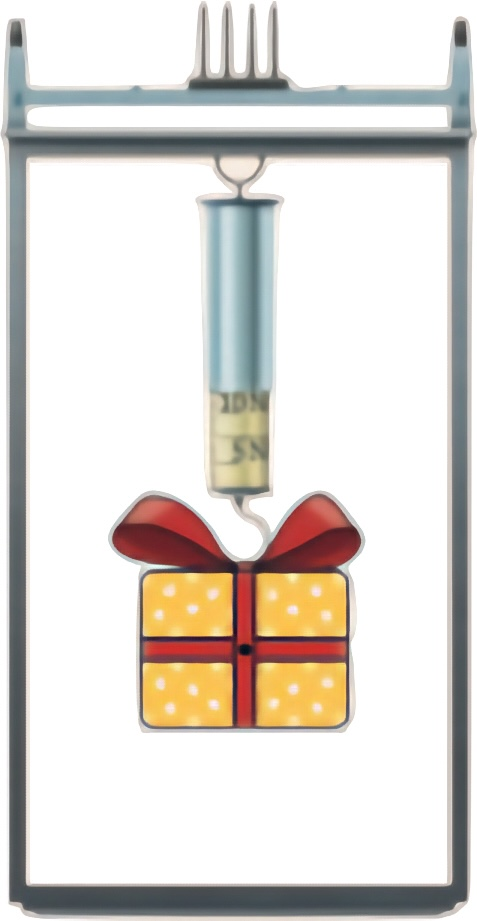
\includegraphics[width=\textwidth]{dyn/exercises/9p143}%
		} 
\end{minipage}

\end{exercise}
